\chapter{REFERÊNCIAL TEÓRICO}

\section{Aspectos de Segurança da Informação}
FAZER PEQUENA INTRODUÇÃO
\subsection{Descrição Geral}
Quando o termo Segurança da Informação é citado, juntamente à ele algumas palavras são relacionadas, entre elas: \textbf{integridade, confidencialidade e disponibilidade}. Esse conjunto é responsável pelo pilar dos princípios básicos de Segurança da Informação.

De uma maneira clara e mais objetiva, a definição para esses pilares se dão da seguinte maneira.

\begin{itemize}
\item \textbf{Integridade:} é responsável por garantir que as informações armazenadas estejam em conformidade com suas características originais.

\item \textbf{Confidencialidade:} é quem garante que somente pessoas que tenham autorização as informações armazenadas em uma organização tenha acesso para seu devido uso. Algo corriqueiro que acontece em organizações é quando esse pilar é quebrado, ou seja, informações que não deveriam são vazadas.

\item \textbf{Disponibilidade:} é quem vai garantir que as informações estejam acessíveis sempre que necessário, no exato momento em que foi solicitada tal informação.
\end{itemize} 

\subsection{Invasores, Alvos e Motivações}
FAZER PEQUENA INTRODUÇÃO

\subsubsection{Atacantes}
De uma maneira geral, podemos considerar um atacante como um indivíduo mal-intencionado ou bem-intencionado que utiliza seus conhecimentos para comprometer uma determinada rede de computadores.

Eles utilizam o alto conhecimento para criação de ferramentas ou para manipulação de maneira avançada das existentes para otimizarem o ataque à determinada rede de computadores. 

Os indivíduos mal-intencionados utilizam seu alto conhecimento com objetivos ilícitos afim de quebrar os pilares da Segurança da Informação.

Eles podem ser considerados em três tipos:

\begin{itemize}
\item \textit{Script Kiddies:} Considerado um usuário que deseja acesso a um sistema de maneira rápida e fácil. Devido ao fato de possuírem pouco conhecimento, utilizam ferramentas prontas para realização e comprometimento do sistema alvo. São caracterizados pelas ferramentas que utilizam: \textit{scan, exploit, trojan}.

\item \textit{Blackhats:} Esse termo foi dado por Richard Stallman, para caracterizar um indivíduo criminoso que exerce a função de realizar ataques em sistemas e quebrar os pilares da segurança da informação. São usuários avançados e que utilizam seus conhecimentos para praticarem atos ilícitos dentro de organizações.

\item \textit{Whitehats:} Termo empregado aos indivíduos bem-intencionados que praticam ataques em redes de computadores afim de descobrirem novas vulnerabilidades e reportarem aos administradores responsáveis pelo sistema. São usuários que utilizam seu conhecimento corrigindo falhas de \textit{softwares} e agem dentro da ética \textit{hacker}. Muitos deles prestam consultoria as empresas e dão palestras sobre segurança da informação.
\end{itemize}

\subsubsection{Alvos}
Qualquer dispositivo que esteja conectado a \textit{Internet} pode ser alvo de um ataque. Seja ele um computador de mesa, um \textit{notebook}, um celular, \textit{tablet} entre outros. Os atacantes não buscam apenas informações pessoais e sigilosas quando realizam um ataque, eles também utilizam os alvos como ponte para novos ataques.

\subsubsection{Motivações}
A vontade em demonstrar poder é considerada uma das principais motivações que levam um atacante a invadir um sistema. Querer mostrar que determinadas organizações possuem vulnerabilidades aumenta ainda mais o seu ego.

Diversos ataques são provenientes de grupos que praticam ações ilícitas, e o prestígio perante outros atacantes levam o indivíduo mal-intencionado a realizar ataques.

Outro motivo bastante comum é quando envolve dinheiro. Muitos atacantes são levados pelo lado financeiro em aplicar golpes para obter informações confidenciais de uma determinada organização.

Outros motivos como diversão, ideologia e inclusão em grupos sociais levam o atacante a praticarem esses tipos de ações. 

\section{Principais tipos de ataques e ameaças}
O CERT.br (Centro de Estudos, Resposta e Tratamento de Incidentes de Segurança no Brasil) vem desde o ano de 1999 analisando atividades na \textit{Internet}. A figura abaixo mostra os principais tipos de ataques reportados no ano de 2015.

\begin{figure}[!h]
\centering
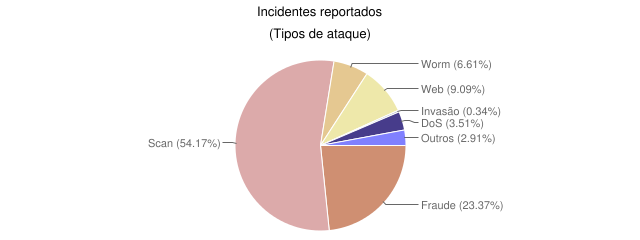
\includegraphics[width = 16cm]{tipos-ataque.png}
\caption{Fonte: CERT.br, 2015.} 	
\end{figure}

A seguir serão mostrado com mais detalhes os principais ataques que foram reportados ao CERT.br, lembrando ao leitor que não são somente esses tipos de ataques que uma organização pode receber.

\begin{itemize}
\item \textit{Worm:} Programa considerado um hospedeiro. É projetado com o intuito de tomar ações que maliciosas que prejudiquem um sistema.

\item \textit{DoS:} Conhecidos como Ataques de Negação de Serviços esse tipo de ataque o atacante utiliza ferramentas com o intuito de retirar do ar um serviço, um computador ou uma rede.

\item \textit{Web:} Esse tipo de ataque visa servidores \textit{Web}, são ataques que resultam em desconfigurações de páginas da \textit{Internet}.

\item \textit{Scan:} Os ataques mais utilizados por \textit{Script-Kiddies} que utilizam para varrer uma rede de computadores. Essa varredura é realizada em portas para verificar quais serviços estão ativos. 

\item Fraude: Segundo o dicionário da língua Portuguesa é o ato ilícito, enganoso, de má-fé com o objetivo de lesar alguém. 

Na computação é empregado em tentativas de fraudes, onde utiliza-se meios para obter informações de maneira ilícita.

\item Outros: Incidentes que não se enquadram nas categorias anteriores.
\end{itemize}

\section{Ferramentas e Componentes de Segurança}
FAZER PEQUENA INTRODUÇÃO 

\subsection{IDS - Sistema de Detecção de Intrusão}
Conhecidos como IDS (\textit{Intrusion Detection System}), esses sistemas trabalham monitorando os eventos que ocorrem dentro de uma rede de computadores, estão presentes nesses eventos as tentativas fracassadas de \textit{login} de um determinado serviço como por exemplo. O objetivo principal desse mecanismo é garantir a segurança da rede, onde são utilizados meios que sejam capazes de prevenir e detectar intrusões de indivíduos mal-intencionados que queiram destruir os pilares da Segurança da Informação (integridade, confidencialidade ou disponibilidade).

Conforme destacam Carissimi, Rochol e Granville (2009) os \textit{IDS} atráves dos \textit{logs} que são deixados no sistema, conseguem identificar eventos que sejam considerados anormais dentro de uma rede, esses eventos anormais podem ser desde uma tentativa de intrusão por algum indivíduo mal-intencionado, ou até mesmo algum download que esteja aumentando o tráfego da rede. Após essa detecção, alertas são disparados como aviso para os administradores de rede. O mais importante contudo é constatar aos administradores de redes que esses tipos de sistemas são muito das vezes um pouco complexo de configura-los.

É interessante, aliás, afirmar que os recursos computacionais a cada dia vem evoluindo mais e mais, organizações cada vez mais necessitam manter a segurança de seus sistemas em conformidade com os pilares da Segurança da Informação. Uma das maneiras de evitar que dados sejam vazados, arquivos sejam perdidos, é utilizar-se desses meios para poder detectar intrusos antes mesmo de uma invasão. 

Recursos computacionais que impedem a ação de indivíduos mal-intencionados em uma rede estão cada vez mais presentes no mercado. Portanto ainda assim é difícil deixar que sua rede ou seu sistema fique longe dessas ameaças ou de vulnerabilidades presente em \textit{softwares}. Uma das formas criadas para que esse tipo de intrusão deixe de acontecer é implementando sistemas de prevenção que impeçam as tentativas de intrusão. (MARCELO e ALVES, 2003).

\subsubsection{Tipos de IDS}
Os \textit{IDS} podem ser classificados em tipos quanto à sua arquitetura. A seguir serão abordadas dois tipos mais utilizados: Sistemas de Detecção de Intrusão baseados em \textit{Host (HIDS)} e Sistemas de Detecção de Intrusão baseados em Rede (\textit{NIDS}).

\subsubsection{Sistemas de Detecção de Intrusão baseados em \textit{Host}}
Esse tipo de \textit{IDS} é instalado dentro de uma máquina que faz a função de servidor dentro de uma rede. Por estarem instalados em um servidor, não se faz necessário o monitoramento em usuários da rede (MARCELO e ALVES, 2003).

O Sistema Operacional em uso será analisado, como seus eventos, seus \textit{logs} gerados, seus eventos de aplicação. O mesmo também irá bloquear tentativas de ataques que o \textit{firewall} deixou a desejar. Normalmente se faz o uso desse tipo de \textit{IDS} quando o objetivo é manter a segurança nas informações que estão armazenadas dentro do servidor.

Em sua maioria se faz o uso de algoritmos complexos, pois o mesmo utiliza para detecção de intrusão o método baseado em anomalias, onde um comportamento anormal é analisado e identificado como atividade suspeita. Um exemplo clássico é quando diversas tentativas de \textit{logins} são realizadas sem sucesso seguidamente (MARCELO e ALVES, 2003).

\begin{figure}[!h]
\centering
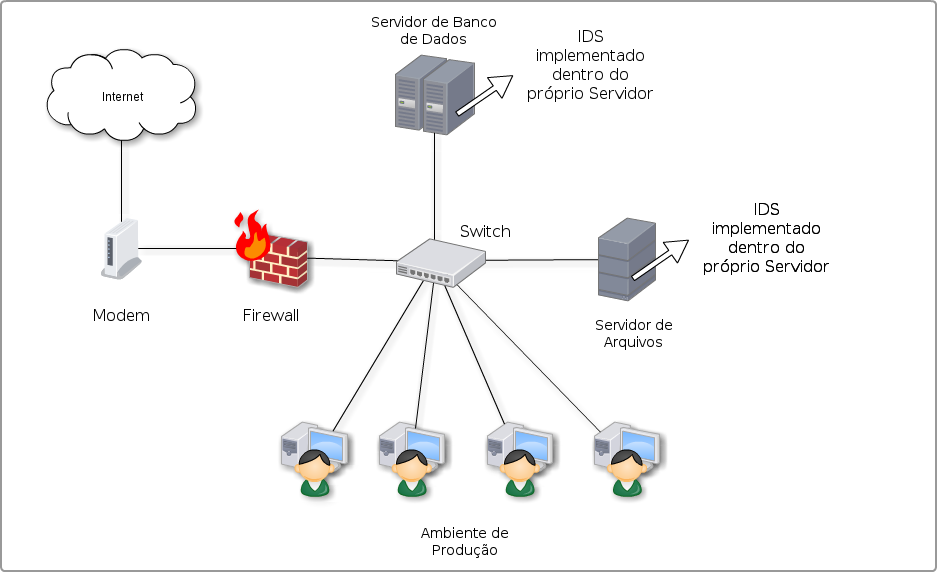
\includegraphics[width = 15cm]{HOST.png}
\caption{\textit{IDS} baseado em \textit{Host}} 	
\end{figure}

\subsubsection{Sistemas de Detecção de Intrusão baseados em Rede}
Esse tipo de \textit{IDS} diferente do baseado em \textit{Host} que monitora um único servidor, ele vai monitorar e analisar todo o comportamento no tráfego da rede. São configurados em pontos estratégicos na rede para detectar todas as atividades suspeitas. 

Eles são configurados para receberem todo o tráfego de entrada e saída afim de detectarem atividades suspeitas. Para isso são configurados em modo promíscuo para analisarem em tempo real o tráfego de rede. Eles operam na camada de rede do modelo \textit{OSI} e por isso são independentes da arquitetura do Sistema Operacional (MARCELO e ALVES, 2003).

\begin{figure}[!h]
\centering
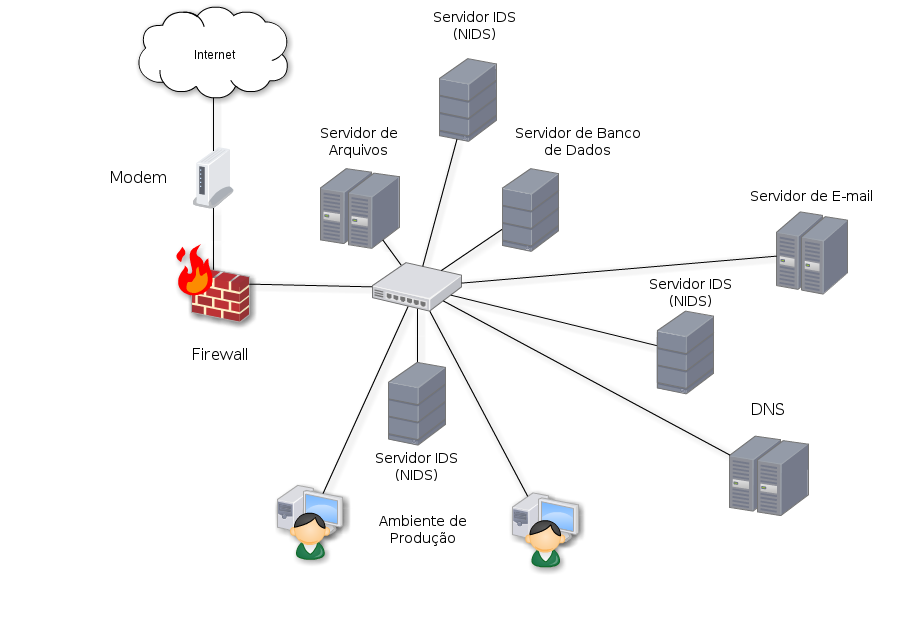
\includegraphics[width = 15cm]{NIDS.png}
\caption{\textit{IDS} baseado em Rede} 	
\end{figure}

\subsubsection{Tipos de Detecção}
\begin{itemize}
\item \textbf{Baseado em assinaturas:} Nesse tipo de detecção é utilizado uma base de dados com assinaturas de ataques conhecidos e armazenados no \textit{IDS} que está em uso. Após um certo comportamento passar pelo tráfego do \textit{IDS}, é feito então uma comparação com as assinaturas existentes no mesmo, e se caso o ataque for um padrão já conhecido, um evento é gerado informado ao administrador que existe um possível ataque.

Para Mohammed e Rehman (2015) uma assinatura é um padrão já existente e está servindo como base para análise de padrões anormais que irão acontecer. Por exemplo, a grande maioria dos anti-vírus utilizam para detecção de \textit{malwares} um padrão de assinaturas. Em sua base de dados está armazenada essa ameaça e quando ela novamente surge é então detectada graças a assinatura armazenada.

A grande desvantagem ao utilizar-se desse meio para detecção de intrusão, é o fato que diversos novos ataques são criados. Quando um novo tipo de intrusão surgir, infelizmente esse método não será viável, pois em sua base de assinaturas só será possível conhecer ataques conhecidos.

\item \textbf{Baseado em anomalias:} Nesse método é identificado comportamentos anormais em uma rede. Mas para a construção desses comportamentos o \textit{IDS} monta um perfil rotineiro da rede, onde por exemplo verifica quais protocolos são utilizados, quais portas são mais utilizadas para conectar à serviços, qual é largura da banda utilizada, entre outros. Após a montagem do perfil, os \textit{IDS´s} monitoram a rede atrás de comportamentos que não se enquadram no perfil montado e sejam considerados anormais. 

As grandes vantagens ao utilizar-se desse meio é que eles são capazes de identificar os comportamentos anormais na rede e detalhar sintomas de um possível ataque. Eles também conseguem produzir informações que podem ser futuramente utilizadas como assinaturas para novos ataques. (MARCELO e ALVES, 2003).

Por outro lado existem as desvantagens. A principal desvantagens é em relação ao grande número de alarmes falsos que o \textit{IDS} irá gerar. Por exemplo, é difícil analisar minuciosamente o comportamento de um usuário. O mesmo pode em um dia fazer diversos \textit{downloads} e sobrecarregar a rede, ou então ele pode ser infectado por um \textit{malware} que esgote os recursos da rede, ou que envie uma grande quantidade de \textit{e-mails} em forma de \textit{spam}.
\end{itemize}

\subsection{Firewall}
Podemos imaginar um \textit{Firewall} sendo um conjunto de sistemas e regras que definem a segurança das informações em uma rede de computadores. Esse conjunto vai servir como uma barreira, impedindo o acesso não autorizado de tráfego de dados, bloqueando os dados e acessos indesejados. Para uma compreensão melhor, de uma maneira abstrata, imagine o \textit{Firewall} como a porta giratória de um banco, onde para poder entrar é necessário obedecer determinadas regras, como não portar objetos suspeitos, em certas condições se identificar, aguardar outra pessoa entrar.

Como bem nos assegura Carissimi, Rochol e Granville (2009), pode-se dizer que um \textit{Firewall} é um conjunto de regras que controlam a comunicação de tráfego que entra e saí de uma rede. Nesse contexto, fica claro que ele aplica regras de filtragem na rede, onde essas regras são aplicadas em diferentes camadas de protocolo. Eles podem ser implementados de diferentes formas, cabe ao administrador de rede escolher qual a maneira que mais se adequa à seu ambiente. Eles podem ser implementados desde \textit{softwares} instalados em um computador ou até mesmo roteadores que desempenham tal função.

Segundo Kurose e Ross (2010) um \textit{Firewall} é considerado um sistema de \textit{hardware} em conjunto com um \textit{software}. A sua principal função é isolar todo o tráfego indesejado que chega até a rede interna. Esse isolamento é definido pelo administrador de rede, onde o mesmo poderá controlar todo o fluxo de tráfego que entra dentro da rede interna. Ainda para esses autores, os \textit{Firewall's} podem ser definidos em três tipos: filtros de pacotes tradicionais, filtros de estado e \textit{gateways} de aplicação.

Com base nas informações dos autores citados acima podemos compreender que a principal característica de um \textit{Firewall} é impedir o tráfego indesejado de um computador ou na rede, para isso ambos os autores possuem a mesma ideia acerca do isolamento do tráfego que não é desejado. Como nos assegura os autores, com o impedimento desse tráfego é possível então impedir diversos fatores que prejudiquem a rede, como por exemplo um \textit{malware} que venha a utilizar determinada porta ou serviço para se instalar em um computador sem o consentimento do usuário.

Um dos principais objetivos de um \textit{Firewall} dentro de uma organização é controlar a política de segurança, pois a partir dele é possível controlar serviços, comportamentos e usuários. Computadores conectados dentro da rede poderão ter acessos a serviços externos se o \textit{Firewall} estiver configurado para permitir esses acessos. O comportamento então se engloba na aplicação de regras que são configuradas por administradores de rede que permitem que padrões pré-estabelecidos não sejam violados. Por fim o controle de usuários, são estabelecidos de acordo com a regra de negócio que a organização se encontra. Por exemplo, apenas os gerentes poderão ter acessos as redes sociais, ou apenas usuários autorizados poderão instalar determinados \textit{softwares}.

Ainda para Carissimi, Rochol e Granville (2009) o gerenciamento dentro de uma organização é dado pela política de segurança que a empresa possui, ou seja, para que seja estabelecido um padrão de regras, um modelo de regra de negócio deve ser seguido. Para isso, os controles são definidos levando em conta o controle sobre serviços, comportamento e permissões de usuários. 

O autor deixa claro na citação acima que para implementação de um \textit{Firewall} seguindo as diretrizes de política de segurança, é necessário que a organização tenha uma regra de negócio a ser seguida, somente assim serviços, controle de usuários poderão ser implementados de maneira mais correta e profissional.

Essas informações nos levam a ter uma noção mais ampla do que é um \textit{Firewall}, e qual seu principal objetivo dentro de uma organização, visto que para um funcionamento adequado o bloqueio de tráfego indesejado e maior controle de política de segurança é necessário que a organização se adeque a uma regra de negócio. A seguir veremos com mais detalhes o seu funcionamento, como é composto sua arquitetura e quais os principais tipos de \textit{Firewall}.

\subsubsection{Arquitetura de Firewall}
Em uma organização, os \textit{Firewall´s} podem ser projetados de algumas maneiras, no qual é enquadrado como arquitetura de \textit{Firewall}. Quando o termo arquitetura é mencionado, devemos nos referir a maneira em que ele é implementado dentro de uma rede de computadores. Para isso, existem três tipos básicos de arquitetura.

\begin{itemize}
\item \textbf{\textit{Screened Host:}} A implementação dessa arquitetura, segue um padrão onde existe um computador que é utilizado como função de roteador, no qual é considerado \textit{screening router} e outro computador denominado \textit{bastion host}.

Nesse tipo de arquitetura, a segurança é fornecida através da filtragem de pacotes. Por exemplo, esse filtro empregado é que impede usuários de realizarem conexões diretas com o serviço de \textit{proxy}.

% verificar aqui, pois o texto original é em inglês
O \textit{bastion host} é configurado para permitir conexões vindas da rede interna para acessarem a rede externa. Ele vai atuar como uma camada de segurança a mais dentro da rede, a comunicação com a rede externa ocorre de dentro para fora, ou seja, a rede interna solicita algo, em seguida passa pelo \textit{bastion host}, chega ao \textit{screening router} e por fim até a rede externa e vice-versa. É ele por exemplo, quem vai realizar a entrega de \textit{e-mails} recebidos. (ZWICKY et al., 2000).

Esse tipo de arquitetura oferece a vantagem de possuir uma camada extra de proteção, pois o \textit{screening router} vai trabalhar filtrando os pacotes e redirecionando o tráfego com filtros configurados para o \textit{bastion host}. Para isso é necessário que seja bem configurado, pois senão poderá comprometer a segurança da rede, ou então qualquer erro pode enviar pacotes indevidos para a rede interna. 

A figura a seguir demonstra uma versão simples de uma arquitetura \textit{Screened Host}.

\begin{figure}[!h]
\centering
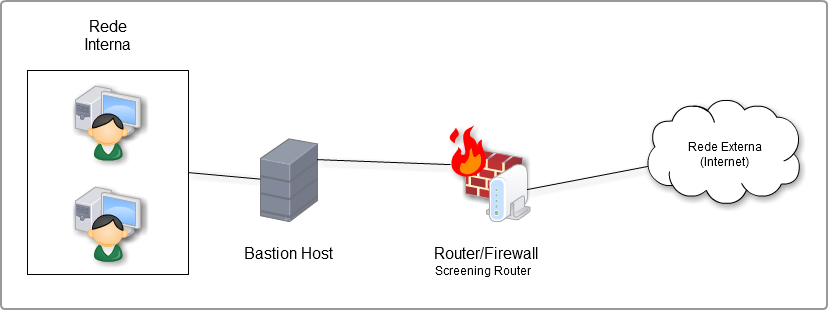
\includegraphics[width = 15cm]{ScreenedHost.png}
\caption{Arquitetura \textit{Screened Host}} 	
\end{figure}

\item \textbf{\textit{Dual-Homed Host:}} Nesse tipo de arquitetura o \textit{Firewall} implementado é formado por um servidor com duas interfaces \textit{ethernet}.

Por existir essas duas interfaces de rede, não existe outro caminho de comunicação, portanto todo o tráfego deve passar pelo \textit{Firewall}. Como bem nos assegura Nakamura (2007) esse tipo de arquitetura fornece serviços através da utilização de \textit{proxies}, ou seja, para que o usuário acesse a rede externa (\textit{Internet}), é necessário que ele se conecte primeiro ao \textit{host dual-homed}.

A grande vantagem ao utilizar essa arquitetura é o controle no tráfego de dados. Porém sua configuração devem ser digamos que perfeita, pois qualquer má configuração pode comprometer a rede toda. É indicado principalmente em organizações que possuem um tráfego baixo para \textit{Internet}, que não possuam dados valiosos, ou que querem supervisionar minuciosamente o tráfego de \textit{Internet}.

A figura abaixo demonstra sua configuração.

\begin{figure}[!h]
\centering
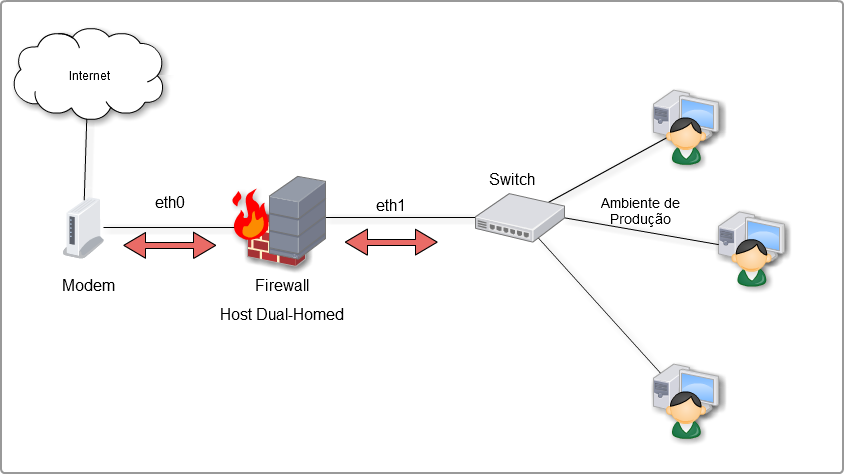
\includegraphics[width = 15cm]{DualHomed.png}
\caption{Arquitetura \textit{Dual-Homed Host}} 	
\end{figure}

\item \textbf{\textit{Sreened Subnet:}} Considerada a arquitetura mais complexa e mais cara de implementar, é também a mais segura. 

Segundo Nakamura (2007), a utilização de uma zona desmilitarizada - \textit{DMZ}, aumenta a segurança em relação ao outros tipos. O \textit{bastion host} graças ao \textit{DMZ} vai ficar em uma zona com mais proteção, utilizando dois filtros.

Na arquitetura \textit{screening router} se o indivíduo mal-intencionado tomasse posse do \textit{bastion host} ele já poderia comprometer a rede interna, nesse caso é diferente, pois o \textit{bastion host} fica em uma zona mais segura, contando com dois filtros. Caso o invasor passe pelo primeiro filtro, ele ainda terá outra tarefa, se aponderar da zona desmilitarizada.

O funcionamento dessa arquitetura se dá graças aos dois filtros, onde o filtro externo permite o tráfego dos serviços que se encontram na zona desmilitarizada e o tráfego das requisições dos usuários internos. Enquanto o filtro externo permite requisições para usuários que estão do lado interno da rede.

A figura abaixo ilustra o funcionamento dessa arquitetura.

\begin{figure}[!h]
\centering
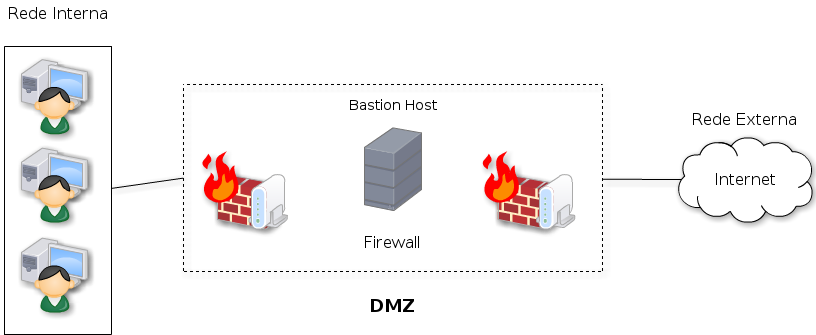
\includegraphics[width = 15cm]{ScreenedSubnet.png}
\caption{Arquitetura \textit{Screened Subnet}} 	
\end{figure}

\end{itemize}

\subsubsection{Tipos de Firewall}
A seguir serão apresentados os principais tipos de \textit{Firewall}, lembrando ao leitor que existem diversos disponíveis no mercado atualmente, aqui veremos os três principais tipos.

\begin{itemize}
\item \textbf{Filtragem de Pacotes \textit{packet filtering:}} Esse tipo de implementação é baseado na técnica de filtragem de pacotes de dados. Essa técnica é relativamente simples, mais ainda assim oferece um nível de segurança quando implementado.

Segundo Nakamura (2007) essa técnica atua na camada de transporte da Pilha \textit{TCP/IP}, onde realiza a decisão de filtros de acordo com as informações relevantes no cabeçalho dos pacotes.

O \textit{Firewall} analisa as informações contidas no pacote e de acordo com as regras pré-estabelecidas libera ou não o pacote. Em determinados casos ele pode arquivar em arquivos de \textit{logs} tarefas ou serviços relacionados, como por exemplo a tentativa de acesso não autorizado em determinado site.

A grande vantagem em utiliza-lo é o fato de ser uma alternativa barata e flexível, visto que o mesmo atua na camada de rede de transporte. A grande maioria de roteadores que atuam como \textit{gateway} dispõe desse tipo de implementação. Por outro lado, o grau de segurança de um pacote não garante tanta segurança, pois um pacote pode ser facilmente falsificado. Além disso esse tipo de implementação não é capaz de diferenciar um pacote verdadeiro de um falso.

A imagem a seguir demonstra sua utilização de uma maneira abstrata.

\begin{figure}[!h]
\centering
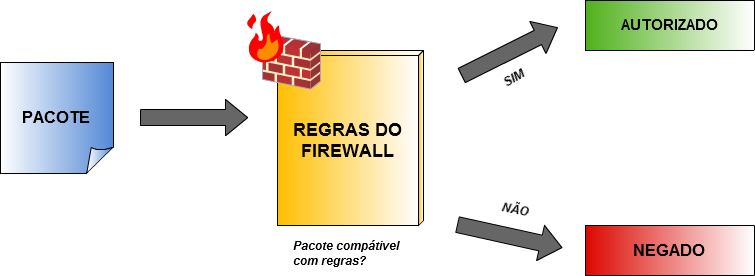
\includegraphics[width = 15cm]{packetfiltering.png}
\caption{Filtragem de pacotes} 	
\end{figure}

\item \textbf{Firewall de aplicação \textit{(proxy services)}:} Esse tipo é conhecido simplesmente por \textit{proxy}. É uma solução que vai atuar como uma ponte entre o usuário e a \textit{Internet}. 

Ele atua recebendo requisições do cliente (usuário), em seguida o \textit{proxy} vai atuar como um cliente e solicitar dados para o servidor que está atuando na rede externa. Após receber a resposta do servidor o \textit{proxy} entrega a resposta ao cliente.

Todo o fluxo de dados passa pelo \textit{proxy}, desta maneira é possível criar regras para que determinados acessos sejam impedidos de serem acessados, como por exemplo impedir acessos a endereços externos.

Algumas vantagens ao utilizar-se desse meio são a criação de \textit{logs} do tráfego e de atividades. Ele não permite conexão direta de um usuário da rede interna diretamente com a rede externa. Em contrapartida ele é mais lento que o filtro de pacotes e não conseguem tratar pacotes \textit{ICMP}.

\begin{figure}[!h]
\centering
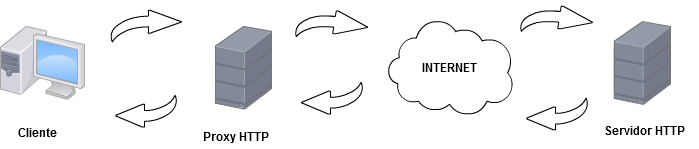
\includegraphics[width = 15cm]{proxyServices.png}
\caption{\textit{Firewall} de Aplicação} 	
\end{figure}

\item \textbf{Inspeção de estados \textit{stateful inspection:}} Considerado por especialistas como uma evolução, esse tipo se enquadra na terceira geração de \textit{Firewall´s}. 

Ele vai rastrear conexões de rede utilizadas pelos aplicativos de rede para encontrar padrões que sejam aceitáveis em suas regras. Quando ele recebe um pacote, ele vai verificar em sua tabela de estados e verificar se tal conexão já foi realizada, caso não tenha sido, esse pacote poderá ser enquadrado em sua política de segurança servindo de parâmetro para o próximo tráfego.

\end{itemize} 
\section{HONEYPOTS}

\subsection{Conhecendo os Honeypots}
Utilizados como "armadilhas", os \textit{Honeypots} servem para atrair indivíduos mal-intencionados que desejam buscar o acesso não autorizado em computadores de determinadas redes que se encontram vulneráveis. São utilizados para serem comprometidos, para que administradores de rede possam fazer uma análise nas informações deixadas por esses indivíduos, para poderem traçar medidas de prevenção de segurança.

Como bem nos assegura Wrightson(2014), os \textit{Honeypots} são propositalmente configurados com vulnerabilidades específicas para que o atacante, ou seja, o indivíduo mal-intencionado, seja atraído. Afinal, esse ambiente agora possui vulnerabilidades que são de interesse para o atacante. Esse ambiente preparado, é capaz de fornecer provas de tentativas de ataques, pois foram configurados como armadilhas, e com esse propósito.

É notável que a citação acima demonstra que seu uso deve ser utilizado de maneira proposital, pois é uma ferramenta utilizada para o estudo, e com esse estudo conseguir adotar medidas de prevenção. Obviamente denota-se que se for configurado de maneira incorreta, ou cair em mãos de indivíduos despreparados, isso resultará em um caminho mais fácil para o atacante, no qual será possível comprometer toda a rede.

Por ser um recurso computacional exposto de maneira proposital por administradores de rede para serem comprometidos, isso nos leva a entender que o uso desse método é possível coletar informações adicionais para a tomada de decisões de segurança em uma rede. (SPITZNER, 2003).

Os bens mais valiosos dentro de ambientes corporativos, são suas informações. As definições de Wrightson (2014) e Spitzner (2003) nos levam a entender que se forem utilizados de maneira correta, as armadilhas criadas com o uso de \textit{Honeypots} podem servir para os administradores de rede tomarem atitudes e medidas de prevenção para segurança e sigilo dessas informações.

Em ambientes corporativos o termo \textit{hacker} significa prejuízo. Mesmo que o seu real significado, empregado pela mídia, não seja esse. A falta de implantação de sistemas e medidas de segurança utilizadas por administradores de rede é o fator que implica o termo \textit{hacker} a tomar esse caminho. As invasões, os vírus e o roubo de informações sigilosas são um pesadelo para qualquer tipo de organização, e isso trás um potencial devastador para as organizações despreparadas de políticas de segurança adequadas.

\begin{quote}
É necessário implementar e manter atualizadas medidas de segurança técnicas e de procedimentos com boa relação custo-benefício para determinar a identificação dos usuários, implementar a devida autenticação e impor direitos de acesso. (FONTES, 2012, p.61)
\end{quote}

O autor deixa claro na citação acima que medidas de segurança e procedimentos devem e precisam ser implementados. Esse é o motivo pelo qual é importante frisar esse ponto, uma vez que, uma falha no sistema pode comprometer toda a segurança da organização, trazendo prejuízos imensuráveis.

Com essa visão pode-se ter um conhecimento mais amplo do que são \textit{Honeypots}, e quais os fundamentos de utilizar suas implementações como medida de prevenção. Obviamente que uma série de outras medidas precisam serem adotadas para impedir que esses indivíduos se apoderem do sistema, porém a utilização de \textit{Honeypots} visa ajudar os administradores a entender como funciona o comportamento desses indivíduos, e auxilia-los a tomarem medidas de prevenção.

\subsection{Classificação de Honeypots por níveis de interatividade}
\textit{Honeypots} possuem níveis de interatividade que podem ser definidos por características próprias de cada nível. A facilidade na manutenção, o nível de segurança e o custo de implementação são alguns dos exemplos de características que cada nível de interatividade pode apresentar. Nas sessões abaixo serão mostrados características de cada um dos três níveis de interação: \textbf{baixa, média e alta}.

\subsubsection{Honeypots de baixa interatividade}
\textit{Honeypots} de baixa interatividade, são aqueles que emulam serviços ou até mesmo Sistemas Operacionais dentro de uma determinada rede. O nível de interatividade entre o sistema emulado e o atacante é baixo. A implementação desse nível, exige um risco pequeno e também um baixo custo de implementação.

Como bem nos assegura Batistela e Trentin (2009), \textit{Honeypots} de baixa interatividade trás uma visão limitada de interação com o atacante, além disso, é considerado o tipo que trás menor manutenibilidade em aspectos de configuração, segurança e baixo custo. Exemplos de serviços básicos que podem ser emulados, são o \textit{FTP - File Transfer Protocol} e o \textit{Telnet}.

Apesar do nível de interação ser considerado baixo com o atacante, se o objetivo do administrador de rede for apenas visar a facilidade de configuração e o baixo custo de implementação, os \textit{Honeypots} de baixa interatividade são os mais ideais para o ambiente. Sua implementação a maioria das vezes é por meio de aplicativos instalados e pré-configurados, tornando o ambiente restrito a interações do atacante.

Ao executar tarefas simples, como por exemplo, monitorar as portas de uma determinada rede, a fim de encontrar portas abertas, esse tipo de \textit{Honeypot} ficará restrito a pilha \textit{TCP/IP}. Alguns tipos de \textit{Honeypots} com esse nível de interatividade podemos citar \textit{Specter, Honeyd e KFSensor} (MARTIM; PAULO \textit{apud} PROVOS).

Dentre as vantagens como a baixa manutenibilidade, citada pelos autores, desvantagens também existem, como a limitação de análises através de \textit{logs} gerados, o que dificultará uma formulação mais precisa do perfil do atacante. Esse tipo de \textit{Honeypot} é projetado para capturar atividades maliciosas conhecidas, sendo assim, com alguns comandos o atacante pode perceber a armadilha, e com pequenos comandos descobrir que está sendo alvo de investigação.

\textit{Honeypots} de baixa interação explora a grande vantagem em não permitir a interação do atacante diretamente com a rede, não trazendo nenhum risco e nem servindo de ponte para outros tipos ataques realizados pelo indidíduo mal-intencionado.

Segundo Batistela e Trentin (2009) a grande vantagem em não permitir que o atacante tenha contato direto com a rede e não realize novos ataques a partir dessa interação, é isso que motiva os administradores de redes ou organizações a começarem inicialmente trabalharem com esses tipos de \textit{Honeypoyts}.

O autor deixa claro ao citar a vantagem em utilizar esse mecanismo de baixa interação, principalmente para quem está iniciando, visto que o mesmo não comprometerá a rede e nem servirá de base para outros ataques. Apesar de possuírem a desvantagem em relação a análise de \textit{logs}, para quem deseja implementar um recurso de segurança adicional na organização, afim de detectar atividades maliciosas, e com custo de implementação baixo, esses tipos de \textit{Honeypots} são os mais indicados.

Diante das informações expostas, pode-se verificar a finalidade de uso desse tipo de interação. É mostrado que esse nível quando utilizado, permite ainda menos risco a rede, facilidade na configuração e na manutenção como principais vantagens. É apresentado as desvantagens no uso desse tipo de interação, como a falta de informações suficientes gerados pelo serviços de \textit{logs}.

\subsubsection{Honeypots de média interatividade}
Assim como \textit{Honeypots} de baixa interatividade, esse tipo de \textit{Honeypot} irá emular serviços com vulnerabilidades, porém com uma gama maior em detalhes, mas ainda assim não deixa de ser um sistema real. Esse tipo de interatividade consegue obter mais dados e informações do atacante, pois o mesmo possui interação maior com o sistema, os serviços que são emulados durante essa interação conseguem responder a requisições dos atacantes, como se fossem serviços reais disponibilizados. Graças a esse tipo de interação o atacante fica em um ambiente falso, e em momento algum terá contato com o sistema operacional real.

Para Alves e Pitanga (2003) diz que esse tipo de interação pode nos trazer mais informações acerca do invasor, pois aqui é emulado com mais precisão os serviços. Esses serviços respondem de maneira falsa, fazendo assim o invasor achar que está em um sistema operacional real. Esse tipo de \textit{Honeypot} consegue nos trazer mais informações das técnicas utilizadas pelo invasor. Apesar desse tipo oferecer mais detalhes, ele também nos trás um risco maior, pois se o invasor consegue descobrir qualquer má-configuração, ele é capaz de invadir o sistema operacional onde o serviço está sendo emulado.

Sabendo ainda que esse tipo de \textit{Honeypot} podem trazer riscos a infra-estrutura da rede,é necessário então ter cautela para esse tipo de implementação, ainda mais se forem operados por usuários e administradores iniciantes e inexperientes, pois um descuido podem comprometer a rede. Nesta perspectiva entendemos que o nível de interação desse \textit{Honeypot} podem nos trazer mais benefícios de estudo e comportamento do que os \textit{Honeypots} de baixa interatividade, pois aqui as técnicas utilizadas pelos invasores serão trazidas com mais detalhes.

Esse tipo, pode ainda fornecer maior interatividade com o atacante, pois é possível utilizá-lo através de ferramentas que o próprio Sistema Operacional \textit{Unix} oferece, o \textit{chroot}. Ele é uma operação no qual será mudado o diretório de root do processo corrente e de seus processos filhos, ou seja, ele permite transformar um diretório no seu diretório raiz atual. Assim é possível criar um sistema virtual aninhado com o real. (BATISTELA; ANTÔNIO, 2009).

FALTA TERMINAR.

\subsubsection{Honeypots de alta interatividade}
Segundo Marcelo e Alves (2003) os \textit{Honeypots} de alta interatividade são Sistemas Operacionais implementados e configurados com falhas reais, e não com falhas emuladas, como os \textit{Honeypots} de baixa e média interatividade. Essas falhas são serviços instalados e configurados em um ambiente real para servir de isca para o invasor.

Como bem nos assegura Assunção (2009), os \textit{Honeypots} de alta interatividade, se forem configurados de maneira correta, além de conseguir capturar todo o comportamento do indivíduo mal-intencionado, também conseguem ficar imperceptível para o invasor, pois é semelhante ao sistema real onde o mesmo se encontra.

Para Spitzner (2002) os \textit{Honeypots} de alta interatividade facilita na captura de informações mais precisas de um invasor, pois através de mecanismos implantados podemos estudar o comportamento do indivíduo para traçar medidas de prevenção de segurança. Porém esse tipo de interatividade é considerado o mais difícil de ser implementado, e além da dificuldade, apresenta riscos maiores ao ambiente, e um custo mais elevado.

Como pode-se verificar, os \textit{Honeypots} de alta interatividade podem ser demorados para serem implementados, mas é evidente que se forem aplicados de maneira correta podem ser utilizados para coletarem com mais precisão as informações deixadas por invasores.

Eles funcionam na maioria das vezes em um ambiente controlado, é estruturado em uma arquitetura de rede controlada, ou seja, onde possa ser monitorado pelo administrador de rede. Cita-se, como exemplo, a criação de um \textit{Firewall} que aceite o tráfego de entrada e controle o tráfego de saída juntamente com um Sistema de Detecção de Intrusão.

Nesse sentido, os \textit{Honeypots} de alta interatividade permite que serviços reais sejam comprometidos. Essa ferramenta configurada corretamente pode ficar imperceptível ao invasor, nos trazendo com precisão o comportamento de indivíduos mal-intencionados.

Logo, é importante compreender que apesar da complexidade, do tempo, e do custo de implementação, esse ambiente consegue nos trazer com mais detalhes o comportamento de invasores. Porém se for mal configurado, ou cair em mãos de indivíduos sem o conhecimento necessário, o risco de comprometimento da rede aumenta, servindo por exemplo, de base para novos ataques. Nesse sentido, vamos exemplificar os \textit{Honeypots} de alta interatividade como um serviço real que pode ser configurado e comprometido para servir de isca para capturar informações com precisão de indivíduos mal-intencionados.

% FALAR DISSO SE DER TEMPO
%\section{Localização dos Honeypots}
%Um fator importante durante a implementação de \textit{Honeypots} que todo administrador de rede deve saber, é quanto a sua localização no ambiente de rede.%
\section{Vantagens e Desvantagens no uso de Honeypots}
FAZER UMA PEQUENA INTRODUÇÃO!
\subsection{Vantagens}
Segundo Mohammed e Rehman (2015) as vantagens no uso de \textit{Honeypots} é a simplicidade em fornecer informações que você precisa. A grande dificuldade que a comunidade de segurança encontra, é a falta, ou limitação dos recursos dos sistemas que são implementados em uma organização. Por exemplo, quando você implementa um \textit{firewall} em uma rede, e o mesmo fica sobrecarregado, suas tabelas de conexões começam a esgotar seus recursos e bloquearem conexões que não deveriam. 

Como bem nos assegura Spitzner (2002), outras vantagens são consideradas importantes, entre elas a capacidade em não utilizar-se de muitos recursos computacionais. Diferente de um \textit{IDS} (Sistema de Detecção de Intrusão) onde o seus sensores podem sofrer dificuldades para captar o grande volume de dados e analisar os pacotes, um \textit{Honeypot} não sofre com isso, pois os recursos utilizados não serão sobrecarregados, pois eles só capturam informações de tráfegos de rede que são dirigidas à ele. Outra vantagem é o pouco investimento em \textit{Hardware} que necessita ser investido. Para o funcionamento adequado não é necessário a utilização de grandes computadores com tecnologia de ponta, equipamentos com pouca memória \textit{RAM}, pouco espaço de armazenamento em disco já é possível a implementação.

Para Simões e Filho (2009) as vantagens no uso de \textit{Honeypots} facilita a diminuição de custos de implementação e custos de manutenção. Um \textit{Honeypot} pode ser implementado utilizando-se máquinas virtuais, além do custo ser muito atrativo, com uma, ou duas máquinas é possível criar diversos cenários interessantes para atrair indivíduos mal-intencionados. Além do custo, com a utilização de \textit{Honeypots} virtualizados você pode contar com diversos sistemas operacionais rodando em uma única máquina. Outra vantagem no uso de \textit{Honeypots} virtualizados é a flexibilidade quando o mesmo é comprometido. Em poucos minutos é possível restaura-lo para uma imagem criada anteriormente.

Como pode-se verificar, diversas vantagens envolvem a utilização de \textit{Honeypots}. Evidentemente a sua aplicação pode ser utilizada em ambientes corporativos que não possuem condições para investimento em sistemas de segurança mais robustos.

Cita-se, como exemplo, imagine uma pequena organização, onde ela está crescendo e sendo visada no mercado, porém a mesma não possui ainda condições de implementar sistemas de segurança de alto custo. Uma boa solução seria a implementação de \textit{Honeypots} para verificar quais técnicas e meios os indivíduos mal-intencionados utilizam-se para tentar se apossar de seus sistemas. Assim administradores poderão tomar as providências necessárias antes mesmo de sofrerem um ataque que possa prejudicar a organização.

Nesse sentido, o seu uso serve como um meio para auxiliar na proteção de ambientes que não possuem condições para investimento em sistemas robustos de segurança da informação, servindo como uma justificativa para determinados investimentos na área da segurança da informação.

\subsection{Desvantagens}
Ao ser citado acima as vantagens ao utilizar-se esses sistemas como auxilio na melhoria de segurança de redes em organizações, a seguir serão mostrada algumas desvantagens que acerca esse tipo de implantação. Compreender isso é um fator muito importante na tomada de decisões de administradores de rede, pois assim será possível identificar e verificar se realmente a implantação de \textit{Honeypots} como ferramenta de auxilio para segurança em redes de computadores é um método eficaz e conveniente.

O mais preocupante, contudo, é constatar que se implementado de maneira incorreta, ele pode trazer grandes riscos para organização, como bem nos assegura Mohammed e Rehman (2015). Se forem sondados ou comprometidos por indivíduos mal-intencionados com bastante experiência, o mesmo pode servir de ponte para o surgimento de novos tipos ataques provenientes da máquina comprometida, tornando-se uma grande ameaça para sua rede. Outra desvantagem relacionada a má configuração é quando administradores utilizam versões comerciais. Essas versões possuem identidades próprias, ou seja, características ou comportamentos que são esperados pelo invasor.

É interessante, aliás, afirmar que essas características de cada um são uma desvantagem, como por exemplo o \textit{Kyppo}, um \textit{Honeypot} que emula vulnerabilidades no serviço \textit{SSH}. Atacantes com mais experiência conseguem facilmente descobrir que estão conectados a esse \textit{Honeypot}. Outro exemplo bastante ocorrido são em servidores web emulados com vulnerabilidades, onde é emulado um servidor \textit{WEB NT ISS}, mas que suas características são de um Servidor \textit{Unix Solaris}. Essas características simples que contradizem as informações são uma grande desvantagem na implementação de \textit{Honeypots}. Mesmo assim parece não haver razão para discordar que os fatores citados como exemplo são aspectos que comprovem suas desvantagens.

\textit{Honeypots} possuem também um campo de visão pouco observado, trata-se inegavelmente pelo fato que o mesmo só consegue analisar as atividades de rede que são dirigidas a ele. Durante a monitoração se nenhum dado de rede chegar até ele, o mesmo não irá gerar nenhum log e nem disponibilizar informação alguma. Se o invasor consegue invadir sua rede e identificar a utilização de \textit{Honeypots}, o mesmo não irá gerar nenhum tipo de atividade para análise, a não ser que o ataque seja feito diretamente nele mesmo. Outra desvantagem quando um \textit{Honeypot} é comprometido, seja pela má configuração por exemplo, é quando após o comprometimento o mesmo serve de apoio para o invasor fazer novos ataques a outras redes ou outros sistemas dentro da própria organização (SPITZNER, 2002).

Com base nas informações dos autores citados acima podemos compreender que desvantagens existem principalmente quando mal configurados ou identificados pelas características que comprovem a existência de \textit{Honeypots}. Além das desvantagens citadas por Spitzner (2002), é necessário também verificar as desvantagens citadas por Mohammed e Rehman (2015), pois uma complementa a outra. É importante ressaltar que administradores de redes procurem também outras fontes de pesquisa, assim, não se baseem somente em uma fonte.

As desvantagens apresentadas exploram as fraquezas ao utilizar-se desse meio. É importante ainda considerar que mesmo comprometidos eles podem ainda serem utilizados para confundir o invasor, e isso é considerado como uma estratégia positiva, pois assim caso o invasor não tenha tanta experiência, ele pode servi-lo como um meio de assusta-lo, fazendo o invasor abandonar o sistema (MOHAMMED; REHMAN, 2015).

O autor deixa bem claro acima que pode ser uma alternativa comprometer um \textit{Honeypot} afim de assustar o atacante, mas pelo receio das organizações em serem alvos de atacantes com mais experiência, o comprometimento não é tão comum, visto que, se comprometido ele pode servir para novos ataques ou comprometimento de toda a estrutura da rede. É por isso que é recomendável a utilização de maneira mais discreta, principalmente por administradores de redes poucos experientes. É válido também deixar claro se o \textit{Honeypot} implementado for para fins de pesquisa ou para o estudo do comportamento do atacante, o seu comprometimento é totalmente válido.

Fica evidente, diante dessas informações que a sua utilização pode trazer diversas desvantagens, e é por isso que o mesmo não deve em hipótese alguma ser utilizado como um mecanismo computacional para substituir outros meios de segurança, como por exemplo, a implementação de \textit{Firewalls}. Esses recursos trabalhados em conjunto com outros meios de segurança agregam diversos valores positivos a uma estrutura de rede.

\section{Ferramentas Utilizadas}
%% Conteudo
AQUI AINDA NÃO SEI AS FERRAMENTAS QUE SERÃO UTILIZADAS
